\documentclass[UTF8,10pt,a4paper]{ctexart}
\usepackage[margin=20mm]{geometry}
\usepackage{graphicx,xcolor,tabularx,booktabs,pdfpages,hyperref}
\definecolor{ink}{HTML}{12313B}\definecolor{teal}{HTML}{008F89}
\hypersetup{colorlinks=true,urlcolor=teal,linkcolor=teal,pdftitle={WorldGuard 参赛提交总册},pdfauthor={零界智行 U406}}
\setlength{\parindent}{0pt}\setlength{\parskip}{5pt}\linespread{1.15}
\begin{document}\pagestyle{empty}
\begin{titlepage}

\includegraphics[height=13mm]{assets/logo.png}\hfill{\small\textcolor{teal}{U406 / UNDERGRADUATE}}
\par\vspace{15mm}
{\Huge\sffamily\bfseries\color{ink}WorldGuard}\par\par\vspace{4mm}
{\LARGE\sffamily\bfseries 面向移动机器人的\\导航测试与验证工作台}\par\par\vspace{4mm}
{\large\color{teal}2026 江苏省 AI＋科学与工程创新实践黑客松}
\par\vspace{10mm}
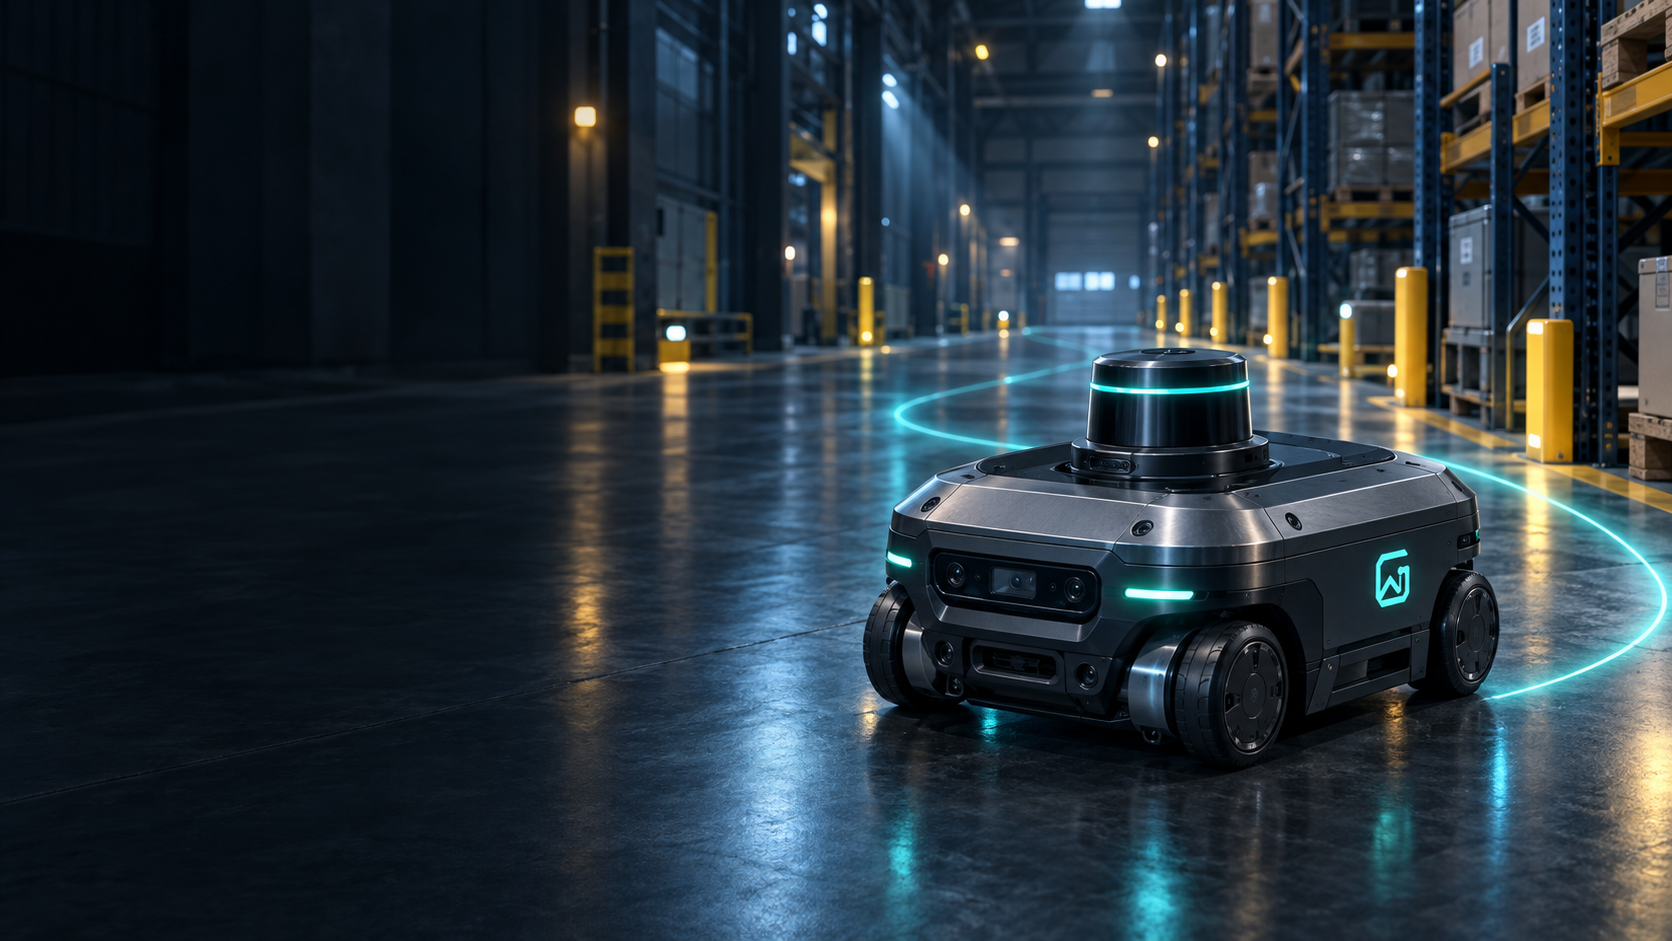
\includegraphics[width=\linewidth]{assets/cover-warehouse.png}\par
{\scriptsize\color{gray}界面概念视觉；真实验证范围为单机器人二维几何仿真。}\par
\par\vspace{7mm}
{\large\bfseries 让失败可复现，让改进有依据。}\par
Agnes 编排测试\quad /\quad 工具独立验收\quad /\quad 保存可复核证据
\par\vfill
\textcolor{teal}{\rule{\linewidth}{1pt}}\par
\begin{tabularx}{\linewidth}{@{}Xr@{}}
\textbf{零界智行}\quad 本科生组 & \textbf{参赛提交总册}\\
束宇涵 · 何万里 · 郑博文 & 2026年10月15日\\
南京大学 / 东南大学 & C4. 无人系统与智能巡检
\end{tabularx}\par
\end{titlepage}
{\small\color{teal}READING GUIDE / 材料导航}\par\par\vspace{4mm}
{\Huge\sffamily\bfseries\color{ink}从结论，到证据。}\par\par\vspace{6mm}
本册汇集项目说明与验证材料。建议先阅读项目报告，再通过工具事件序号、案例文件和哈希定位原始证据。可运行源码与完整日志以同包附件为准。
\par\vspace{5mm}
\begin{tabularx}{\linewidth}{@{}p{13mm}p{40mm}X@{}}\toprule
编号 & 交付模块 & 阅读与核查重点\\\midrule
01 & 项目报告 & 基本信息、问题来源、目标、核心方法与结果\\[3mm]
02 & 技术与复现指南 & AGH、模型环节、工具接口、安装和验证方法\\[3mm]
03 & 可运行作品 & 独立源码附件与公开 GitHub，见下方链接\\[3mm]
04 & 运行与验证证据 & 真实 Host 记录、核心工具链、模型参与、关键配置\\[3mm]
05 & 三类测试样例 & 正常、边界、失败与恢复；均附复核结果\\[3mm]
06 & 成员声明与来源 & 团队职责、独立完成声明、软件与素材使用说明\\[3mm]
07 & 公开内容与视频 & B站公开记录、发布日期截图、04:15 演示视频\\\bottomrule
\end{tabularx}\par
\par\vspace{8mm}
\colorbox{teal!7}{\parbox{0.95\linewidth}{\textbf{代表性验证}\par
2 组真实 Agnes 运行，覆盖 8 个案例。堵路案例原始净空 $-0.230$ m，恢复后 $0.145$ m；原始失败与恢复通过分别保存。三类交付样例均离线重放匹配。}}
\par\vspace{7mm}
\textbf{公开代码与复现}\par
\url{https://github.com/Yu-han-Shu/WorldGuard}\par
\textbf{演示视频与公开项目记录}\par
\url{https://www.bilibili.com/video/BV1dQJ66tEsV/}\par
发布日期：2026-10-15 10:48:05；播放器时长：04:15。
\par\vfill
{\small\color{gray}包内含源码快照、原始结构化证据、三类样例、LaTeX 源文件与文件哈希。当前验证范围为二维仿真，未连接真实机器人。}
\clearpage
\includepdf[pages=-,addtotoc={1,section,1,{项目报告},01-project}]{01-project.pdf}
\includepdf[pages=-,addtotoc={1,section,1,{技术与复现指南},02-technical}]{02-technical.pdf}
\includepdf[pages=-,addtotoc={1,section,1,{运行证据核查指南},03-evidence}]{03-evidence.pdf}
\includepdf[pages=-,addtotoc={1,section,1,{三类测试说明},04-tests}]{04-tests.pdf}
\includepdf[pages=-,addtotoc={1,section,1,{成员声明},05-declaration}]{05-declaration.pdf}
\includepdf[pages=-,addtotoc={1,section,1,{来源与使用说明},06-sources}]{06-sources.pdf}
\includepdf[pages=-,addtotoc={1,section,1,{公开内容与视频},07-public-proof}]{07-public-proof.pdf}
\end{document}
